%%%%%%%%%%%%%%%%%%%%%%%%%%%%%%%%%%%
%This is the LaTeX ARTICLE template for RSC journals
%Copyright The Royal Society of Chemistry 2014
%%%%%%%%%%%%%%%%%%%%%%%%%%%%%%%%%%%

\documentclass[twoside,twocolumn,9pt]{article}
\usepackage{extsizes}
\usepackage[super,sort&compress,comma]{natbib} 
\usepackage[version=3]{mhchem}
\usepackage[left=1.5cm, right=1.5cm, top=1.785cm, bottom=2.0cm]{geometry}
\usepackage{balance}
\usepackage{widetext}
\usepackage{times,mathptmx}
\usepackage{sectsty}
\usepackage{graphicx} 
\usepackage{lastpage}
\usepackage[format=plain,justification=raggedright,singlelinecheck=false,font={stretch=1.125,small,sf},labelfont=bf,labelsep=space]{caption}
\usepackage{float}
\usepackage{fancyhdr}
\usepackage{fnpos}
\usepackage[english]{babel}
\usepackage{array}
\usepackage{droidsans}
\usepackage{charter}
\usepackage[T1]{fontenc}
\usepackage[usenames,dvipsnames]{xcolor}
\usepackage{setspace}
\usepackage[compact]{titlesec}
%%%Please don't disable any packages in the preamble, as this may cause the template to display incorrectly.%%%


\usepackage{epstopdf}%This line makes .eps figures into .pdf - please comment out if not required.

\definecolor{cream}{RGB}{222,217,201}

\begin{document}

\pagestyle{fancy}
\thispagestyle{plain}
\fancypagestyle{plain}{

%%%HEADER%%%
\fancyhead[C]{
\includegraphics[width=18.5cm]{header_bar.pdf}}
\fancyhead[L]{\hspace{0cm}\vspace{1.5cm}\LARGE QuantBio Express}
%\fancyhead[L]{\hspace{0cm}\vspace{1.5cm}\includegraphics[height=30pt]{head_foot/journal_name}}
\fancyhead[R]{\hspace{0cm}\vspace{2.5cm}}
%\fancyhead[R]{\hspace{0cm}\vspace{1.7cm}\includegraphics[height=55pt]{head_foot/RSC_LOGO_CMYK}}
\renewcommand{\headrulewidth}{0pt}
}
%%%END OF HEADER%%%

%%%PAGE SETUP - Please do not change any commands within this section%%%
\makeFNbottom
\makeatletter
\renewcommand\LARGE{\@setfontsize\LARGE{15pt}{17}}
\renewcommand\Large{\@setfontsize\Large{12pt}{14}}
\renewcommand\large{\@setfontsize\large{10pt}{12}}
\renewcommand\footnotesize{\@setfontsize\footnotesize{7pt}{10}}
\makeatother

\renewcommand{\thefootnote}{\fnsymbol{footnote}}
\renewcommand\footnoterule{\vspace*{1pt}% 
\color{cream}\hrule width 3.5in height 0.4pt \color{black}\vspace*{5pt}} 
\setcounter{secnumdepth}{5}

\makeatletter 
\renewcommand\@biblabel[1]{#1}            
\renewcommand\@makefntext[1]% 
{\noindent\makebox[0pt][r]{\@thefnmark\,}#1}
\makeatother 
\renewcommand{\figurename}{\small{Fig.}~}
\sectionfont{\sffamily\Large}
\subsectionfont{\normalsize}
\subsubsectionfont{\bf}
\setstretch{1.125} %In particular, please do not alter this line.
\setlength{\skip\footins}{0.8cm}
\setlength{\footnotesep}{0.25cm}
\setlength{\jot}{10pt}
\titlespacing*{\section}{0pt}{4pt}{4pt}
\titlespacing*{\subsection}{0pt}{15pt}{1pt}
%%%END OF PAGE SETUP%%%

%%%FOOTER%%%
\fancyfoot{}
\fancyfoot[LO,RE]{\vspace{-7.1pt}
\includegraphics[height=15pt]{cc-by-nc-sa.png}}
%\fancyfoot[CO]{\vspace{-7.1pt}\hspace{13.2cm}\includegraphics{head_foot/RF}}
\fancyfoot[CO]{\vspace{-7.1pt}QuantBio Express, vol. 1}
\fancyfoot[CE]{\vspace{-7.2pt}QuantBio Express, vol. 1}
%\fancyfoot[CE]{\vspace{-7.2pt}\hspace{-14.2cm}\includegraphics{head_foot/RF}}
\fancyfoot[RO]{\footnotesize{\sffamily{1--\pageref{LastPage} ~\textbar  \hspace{2pt}\thepage}}}
\fancyfoot[LE]{\footnotesize{\sffamily{\thepage~\textbar 1--\pageref{LastPage}}}}
\fancyhead{}
\renewcommand{\headrulewidth}{0pt} 
\renewcommand{\footrulewidth}{0pt}
\setlength{\arrayrulewidth}{1pt}
\setlength{\columnsep}{6.5mm}
\setlength\bibsep{1pt}
%%%END OF FOOTER%%%

%%%FIGURE SETUP - please do not change any commands within this section%%%
\makeatletter 
\newlength{\figrulesep} 
\setlength{\figrulesep}{0.5\textfloatsep} 

\newcommand{\topfigrule}{\vspace*{-1pt}% 
\noindent{\color{cream}\rule[-\figrulesep]{\columnwidth}{1.5pt}} }

\newcommand{\botfigrule}{\vspace*{-2pt}% 
\noindent{\color{cream}\rule[\figrulesep]{\columnwidth}{1.5pt}} }

\newcommand{\dblfigrule}{\vspace*{-1pt}% 
\noindent{\color{cream}\rule[-\figrulesep]{\textwidth}{1.5pt}} }

\makeatother
%%%END OF FIGURE SETUP%%%

%%%TITLE, AUTHORS AND ABSTRACT%%%
\twocolumn[
  \begin{@twocolumnfalse}
\vspace{3cm}
\sffamily


\noindent\LARGE{\textbf{Who turned out the lights: the shortcomings and successes of a Boolean network model for circadian processes$^\dag$}} \\%Article title goes here instead of the text "This is the title"

 \noindent\large{Adam Gruenbaum and Graham Northrup} \\%Author names go here instead of "Full name", etc.


\noindent\normalsize{The purpose of this paper is to stress test a Boolean network representing circadian rhythms of Arabidopsis. We reproduced a Boolean model for these rhythms obtained from [O. E. Akman, Journal of The Royal Society, 2012.], and subjected the model to situations outside of the standard conditions under which it was designed. We tested it with a variety of photoperiods and submitted it to asynchronous behavior from the light inputs. We found that this particular model doesn't respond well to large changes in photoperiods, but does respond fairly well to asynchronous light node behavior. For a model so small (in terms of number of nodes) it is difficult to rectify these issues, however there are more complex models of the same system that might be more robust to change.} \\%The abstrast goes here instead of the text "The abstract should be..."


 \end{@twocolumnfalse} \vspace{0.6cm}

  ]
%%%END OF TITLE, AUTHORS AND ABSTRACT%%%

%%%FONT SETUP - please do not change any commands within this section
\renewcommand*\rmdefault{bch}\normalfont\upshape
\rmfamily
\section*{}
\vspace{-1cm}


%%%FOOTNOTES%%%

%Please use \dag to cite the ESI in the main text of the article.
%If you article does not have ESI please remove the the \dag symbol from the title and the footnotetext below.
\footnotetext{\dag~Electronic Supplementary Information (ESI) available: https://github.com/gnorthrup/BooleanControl}
%additional addresses can be cited as above using the lower-case letters, c, d, e... If all authors are from the same address, no letter is required

%\footnotetext{\ddag~Additional footnotes to the title and authors can be included \emph{e.g.}\ `Present address:' or `These authors contributed equally to this work' as above using the symbols: \ddag, \textsection, and \P. Please place the appropriate symbol next to the author's name and include a \texttt{\textbackslash footnotetext} entry in the the correct place in the list.}


%%%END OF FOOTNOTES%%%

%%%MAIN TEXT%%%%

\section{Introduction}

Biology is comprised of many processes regulated by the 24hr period of the day, temperature, or other environmental factors. These systems, circadian systems, typically stand on the back of gene regulatory networks (GRNs). A GRN is a group of genes linked by excitatory and inhibitory pathways which, in the circadian case, produce regulated, periodic outputs. These networks can be, and frequently are, modeled using ordinary differential equations (ODEs); however, it has been shown that Boolean networks can perform just as well under certain conditions\cite{digiclocks}.\\

A Boolean network is a way to model systems with binary operators. The vertices (with values 0 or 1) are connected by edges and the corresponding logic gates. The model then uses the values of the connected vertices to generate values at the next time step. A basic 3 node model is shown below along with the accompanying table of values.\\

\begin{figure}[h]
\centering
  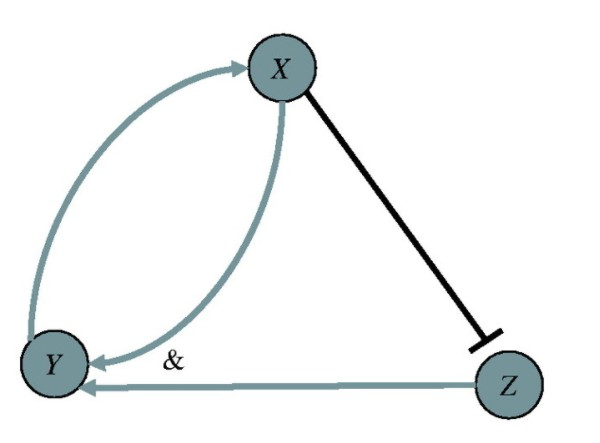
\includegraphics[height=4cm]{basicbool}
  \caption{A simple 3 node Boolean network with no signal delay}
  \label{fgr:example}
\end{figure}

\begin{table}[h]
\small
  \caption{\ The values of X,Y and Z at t+1 given XYZ(t)}
  \label{tbl:example}
  \begin{tabular*}{0.5\textwidth}{@{\extracolsep{\fill}}lll}
    \hline
    XYZ(t) & XYZ(t+1) \\
    \hline
    000 & 001 \\
    001 & 001 \\
    010 & 101 \\
    011 & 101 \\
    100 & 000 \\
    101 & 010 \\
    110 & 100 \\
    111 & 110 \\
    \hline
  \end{tabular*}
\end{table}

The paper put forward by Akman et al. compares the Boolean model to data under rather ideal conditions (synchronous, physically relevant photoperiods),  where it performs rather well. This purpose of this paper is to stress test one of these Boolean models put forth under more extreme conditions and parameterizations to determine the model?s limitations to further understand the Boolean model?s place in GRN modeling.


\section{Methods}

We built a codebase in Matlab to represent and evaluate boolean networks, utilizing a recursive class and evaluation function to represent complex Boolean gates. A matrix was used to represent and store the states of the nodes for each time point, which allowed data from different time points to be accessed during simulation - a necessary piece for signalling delays. Light nodes were implemented to update based on their absolute time step, rather than basing their outputs on stimulus. At the start of any simulation, all states were assumed to be off, and states prior to the start of the simulation (accessed via signalling delays), were assumed to be off. \\
Once this system had been built, it was fairly trivial to implement and simulate a variety of boolean networks. The network we settled on was the 2-loop Arabidopsis model given by Akman et al\cite{digiclocks}. We utilized the logic configuration and signaling delays presented, with a little bit of fiddling to ensure that the model produced the results expected by the paper. Once this model was established it was fairly easy to make changes to the parameters in order to experiment with the model?s response to change. \\
In order to stress the model, we tested all the possible photoperiods that totalled to 24 hours (24hr day, 0 hr night; 23hr day, 1 hr night; etc.) and all the possible photoperiods that totalled to 48 hours. Additionally we ran the model with subsets of lights entirely off (either $L_1$, or $L_2$ \& $L_3$), and tried turning off those subsets of lights in the middle of a simulation. We also tried running the subsets of lights with different periods to examine how the model responded.

\section{Results}

Present your results, divided into sections for different portions of the project. Indicate who worked on each section. Illustrate your results with tables and figures and compare them to previously published results.


\section{Discussion}

Give some big-picture context for your work and speculate on its importance. Describe what you learned from doing this project and what you think about the future directions of this topic. This is where you can use more personal language and say fun things!


\section{Conclusions}
What is your takeaway from this project?


\section{Acknowledgements}

The authors thank Dmitry Kondrashov for his guidance and advice throughout this project.

%%%END OF MAIN TEXT%%%


%The \balance command can be used to balance the columns on the final page if desired. It should be placed anywhere within the first column of the last page.

%\balance

%If notes are included in your references you can change the title from 'References' to 'Notes and references' using the following command:
%\renewcommand\refname{Notes and references}

%%%REFERENCES%%%
\bibliographystyle{rsc} %the RSC's .bst file
\bibliography{BiologyBib} %You need to replace "rsc" on this line with the name of your .bib file


\end{document}
